\documentclass[12pt]{article}

% Packages
\usepackage[margin=6em]{geometry} % 1 cm = 2.84528 em
\usepackage[colorlinks=true,linkcolor=red,urlcolor=blue]{hyperref}
\usepackage{tikz}
\usepackage[backend=bibtex]{biblatex}
\bibliography{sources}
\nocite{*}

\usepackage{lipsum}

% Paragraphs
\setlength{\parindent}{0em}
\setlength{\parskip}{1em}

% Includes
% Includes
\usepackage{amsfonts}
\usepackage{amsmath}
\usepackage{amssymb}
\usepackage{amsthm}
\usepackage{comment}
\usepackage[colorlinks]{hyperref}
\usepackage{letltxmacro}
\usepackage{listings}
\usepackage{stmaryrd}

% Spacing
\let\uspace\undefined
\newcommand{\uspace}{\ensuremath{\ }}

% Numbers
\let\N\undefined
\newcommand{\N}{\ensuremath{\mathbb{N}}}

\let\Z\undefined
\newcommand{\Z}{\ensuremath{\mathbb{Z}}}

\let\Zz\undefined
\newcommand{\Zz}{\ensuremath{\mathbb{Z}^{\geq 0}}}

\let\Zp\undefined
\newcommand{\Zp}{\ensuremath{\mathbb{Z}^{+}}}

\let\Q\undefined
\newcommand{\Q}{\ensuremath{\mathbb{Q}}}

\let\R\undefined
\newcommand{\R}{\ensuremath{\mathbb{R}}}

\let\Rz\undefined
\newcommand{\Rz}{\ensuremath{\mathbb{R}^{\geq 0}}}

\let\Rp\undefined
\newcommand{\Rp}{\ensuremath{\mathbb{R}^{+}}}

\let\C\undefined
\newcommand{\C}{\ensuremath{\mathbb{C}}}

\let\mcal\undefined
\newcommand{\mcal}[1]{\ensuremath{\mathcal{#1}}}

\let\mbb\undefined
\newcommand{\mbb}[1]{\ensuremath{\mathbb{#1}}}

% Grouping
\let\parens\undefined
\newcommand{\parens}[1]{\ensuremath{\left(#1\right)}}

\let\brackets\undefined
\newcommand{\brackets}[1]{\ensuremath{\left[#1\right]}}

\let\braces\undefined
\newcommand{\braces}[1]{\ensuremath{\left\{#1\right\}}}

\let\angles\undefined
\newcommand{\angles}[1]{\ensuremath{\left\langle#1\right\rangle}}

\let\ceil\undefined
\newcommand{\ceil}[1]{\ensuremath{\left\lceil#1\right\rceil}}

\let\floor\undefined
\newcommand{\floor}[1]{\ensuremath{\left\lfloor#1\right\rfloor}}

% Sets and Function Spaces
\let\type\undefined
\newcommand{\type}[3]{\ensuremath{#1 \colon #2 \to #3}}

\let\powset\undefined
\newcommand{\powset}[1]{\ensuremath{2^{#1}}}

\let\mod\undefined
\newcommand{\mod}{\ensuremath{\uspace\mathrm{mod}\uspace}}

\let\ker\undefined
\newcommand{\ker}{\ensuremath{\mathrm{ker}}}

\let\dom\undefined
\newcommand{\dom}{\ensuremath{\mathrm{dom}}}

\let\ran\undefined
\newcommand{\ran}{\ensuremath{\mathrm{ran}}}

\let\im\undefined
\newcommand{\im}{\ensuremath{\mathrm{im}}}

\let\coker\undefined
\newcommand{\coker}{\ensuremath{\mathrm{coker}}}

\let\codim\undefined
\newcommand{\codim}{\ensuremath{\mathrm{codim}}}

% Complex Numbers
\let\Re\undefined
\newcommand{\Re}{\ensuremath{\mathrm{Re}}}

\let\Im\undefined
\newcommand{\Im}{\ensuremath{\mathrm{Im}}}

% Probability
\let\Pr\undefined
\newcommand{\Pr}{\ensuremath{\mathrm{Pr}}}

\let\E\undefined
\newcommand{\E}{\ensuremath{\mathrm{E}}}

\let\Var\undefined
\newcommand{\Var}{\ensuremath{\mathrm{Var}}}

\let\Cov\undefined
\newcommand{\Cov}{\ensuremath{\mathrm{Cov}}}

% Integrals
\let\dee\undefined
\newcommand{\dee}[1]{\ensuremath{\uspace d #1}}

% Linear Algebra
\let\abs\undefined
\newcommand{\abs}[1]{\ensuremath{\left\lvert#1\right\rvert}}

\let\norm\undefined
\newcommand{\norm}[1]{\ensuremath{\left\lVert#1\right\rVert}}


% Computational Complexity
\let\class\undefined % Complexity class
\newcommand{\class}[1]{\ensuremath{\mathbf{#1}}}

\let\prob\undefined % Complexity problem
\newcommand{\prob}[1]{\ensuremath{\text{#1}}}

% Theorem environment
\theoremstyle{plain}
\newtheorem{theorem}{Theorem}

\theoremstyle{plain}
\newtheorem{lemma}{Lemma}

\theoremstyle{plain}
\newtheorem{claim}{Claim}

\theoremstyle{plain}
\newtheorem{fact}{Fact}

\theoremstyle{plain}
\newtheorem{remark}{Remark}

\theoremstyle{plain}
\newtheorem{definition}{Definition}

\theoremstyle{plain}
\newtheorem{example}{Example}

\theoremstyle{plain}
\newtheorem{question}{Question}

% Code environment
\lstdefinestyle{plainsty}{
  basicstyle=\small\ttfamily,
  language=C,
  xleftmargin=\parindent,
  aboveskip=1em,
  belowskip=1em,
  showspaces=false,
  showstringspaces=false,
  keywordstyle = {},
}

\lstnewenvironment{pcode}{\lstset{style=plainsty}}{}

\let\pinl\undefined
\newcommand{\pinl}{\lstinline[style=plainsty]}

\newcommand*{\SavedLstInline}{} % Allows plain code usage in math mode.
\LetLtxMacro\SavedLstInline\pinl
\DeclareRobustCommand*{\pinl}{%
  \ifmmode
    \let\SavedBGroup\bgroup
    \def\bgroup{%
      \let\bgroup\SavedBGroup
      \hbox\bgroup
    }%
  \fi
\SavedLstInline}

\let\ttcode\undefined
\newcommand{\ttcode}[1]{\small{\texttt{#1}}}


% Text markings

\let\tturl\undefined
\newcommand{\tturl}[1]{\href{#1}{\texttt{#1}}}

\let\red\undefined
\newcommand{\red}[1]{\textbf{\color{red}#1}}


% Abbreviations
\let\st\undefined
\newcommand{\st}{\ensuremath{\uspace\colon\uspace}}

\let\ow\undefined
\newcommand{\ow}{\ensuremath{\text{otherwise}}}




\let\company\undefined
\newcommand{\company}{\textbf{Big Tech Company}}

\let\Android\undefined
\newcommand{\android}{Android}

\let\state\undefined
\newcommand{\state}{\ensuremath{\sigma}}

\let\var\undefined
\newcommand{\var}{\ensuremath{x}}

\let\domval\undefined
\newcommand{\domval}{\ensuremath{\mathcal{A}}}

\let\formula\undefined
\newcommand{\form}{\ensuremath{\varphi}}

\let\domform\undefined
\newcommand{\domform}{\ensuremath{\mathcal{F}}}

% Author
\title{The Dangerous Graph}
\author{Anton Xue}
% \date{\today}
\date{}

% Document
\begin{document}
\maketitle

\subsection{Real World Applications?}

A friend working at \company{} talked to me about a problem:
how do we automatically detect crashing errors in \android{} applications?

Users interacts with \android{} applications by touching
the phone's user interface (UI).
Touching the UI in specific ways alters the internal state of the application.
The UI is specified by XML files that (each?) represent a
different display layout.
When specific touches are performed, different displays may be shown.
These display transitions are conditional on the internal state of the
application and the current active display.
What sequence of touches will cause the application to crash?

\subsection{The Problem}
At a high level overview standpoint, there are a number of ways to tackle
this problem: randomized testing,
backwards symbolic execution~\cite{baldoni-backwards},
program slicing~\cite{weiser-slicing}, to name a few.
The techniques that may be applied depends on whether we have
white-box access to the program source code.

The most reliable techniques is also among the hardest to implement, and the
sensible solution is perhaps one of in-depth code analysis.
From personal experience, this is both hard and annoying, so we ignore it,
and try something simpler.

Instead, we pretend that we do not have source code access --- in fact,
we make it even more confusing:
we pretend that we have access to the internal program state, the UI
representation of some sort, and of course a phone with the compiled
application.

We then model this as follows:

\if false
\begin{definition}[Application Graph]
An \textit{application graph} is a directed graph $G = \parens{V, E}$.
Each $v \in V$ corresponds to a UI display, and has a state
$v_\state$ which maps variables to elements in a domain of values $\domval$.
Furthermore, every edge $e = (u, v)$ with tail $u$ and head $v$ has
a corresponding label $e_{\form}$, where $\form \in \domform$ is a
formula in some logical theory $\domform$.
\end{definition}
\fi

\begin{example}[Simple UI]
We push our \LaTeX{} skills to bring you this.

\begin{minipage}{0.5\textwidth}
  \begin{center}
  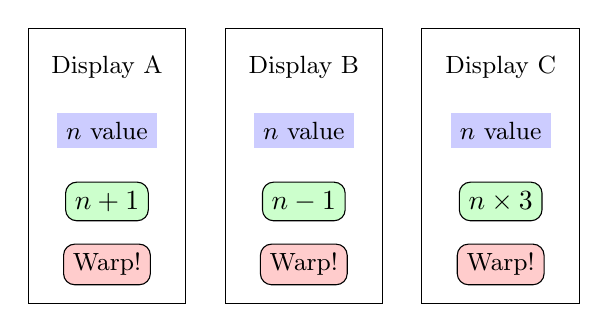
\begin{tikzpicture}
    \draw (0.0, 0.0) -- (2.0, 0.0) -- (2.0, 3.5) -- (0.0, 3.5) -- (0.0, 0.0);
    \draw (2.5, 0.0) -- (4.5, 0.0) -- (4.5, 3.5) -- (2.5, 3.5) -- (2.5, 0.0);
    \draw (5.0, 0.0) -- (7.0, 0.0) -- (7.0, 3.5) -- (5.0, 3.5) -- (5.0, 0.0);

    \node[] at (1.0, 3.0) {{\small Display A}};
    \node[] at (3.5, 3.0) {{\small Display B}};
    \node[] at (6.0, 3.0) {{\small Display C}};

    \node[fill=blue!20] at (1.0, 2.2) {{\small $n$ value}};
    \node[fill=blue!20] at (3.5, 2.2) {{\small $n$ value}};
    \node[fill=blue!20] at (6.0, 2.2) {{\small $n$ value}};

    \node[fill=green!20,draw,rounded corners] at (1.0, 1.3) {$n + 1$};
    \node[fill=green!20,draw,rounded corners] at (3.5, 1.3) {$n - 1$};
    \node[fill=green!20,draw,rounded corners] at (6.0, 1.3) {$n \times 3$};

    \node[fill=red!20,draw,rounded corners] at (1.0, 0.5) {{\small Warp!}};
    \node[fill=red!20,draw,rounded corners] at (3.5, 0.5) {{\small Warp!}};
    \node[fill=red!20,draw,rounded corners] at (6.0, 0.5) {{\small Warp!}};
  \end{tikzpicture}
  \end{center}
\end{minipage}
\begin{minipage}{0.5\textwidth}
\begin{pcode}
// A:
onRed:   set n = n + 1
onGreen: if n mod 5 == 1 then go to B
         if n mod 5 == 2 then go to C
         otherwise do nothing
// B:
onRed:   set n = n - 1
onGreen: if n mod 5 == 0 then go to A
         if n mod 5 == 2 then go to C
         otherwise do nothing
// C:
onRed: n = n * 3
onGreen: if n mod 5 == 0 then go to A
         if n mod 5 == 1 then go to B
         otherwise CRASH
\end{pcode}
\end{minipage}

The state graph is then defined as follows:

\end{example}


\printbibliography


\end{document}
